%-----------------------------------------------------------
% LaTeX template for University of Warwick exams
%-----------------------------------------------------------

% load the uow-exam class, the following options are supported:
% 'answers' shows solutions where specified 
\documentclass[palatino, code, aep]{uow-exam}

\usepackage{fancyeq}
\usepackage{tikz}
\usetikzlibrary{automata, positioning, arrows}

% configure the heading 
\ModuleCode{CS141}
\ModuleName{Functional Programming} % for aep, this should be all caps
\ExamPeriod{Sample 2021}  
\ExamCode{CS1410\_B}
\TimeAllowed{2 hours} % either 2 hours or 3 hours
\QuestionInstructions{There are \textbf{SIX} questions. Candidates should attempt \textbf{FOUR} questions.}
\OtherInstructions{Instructions specific to this module:
\begin{itemize}
    \item The questions are not in order of difficulty.
    \item Unless stated otherwise, you should assume that library functions are defined as shown in the module guide.
\end{itemize}
General exam instructions follow on the next page.}

% use this if your exam paper contains sections or comment it out otherwise
% \NoBreakAfterQuestions

\setminted[text]{fontsize=\small}
\setminted[haskell]{fontsize=\small}
\setminted[bash]{fontsize=\small}
\newcommand{\haskellTopIn}[1]{\mintinline[fontsize=\small]{text}{#1}}
\newcommand{\haskellIn}[1]{\mintinline[fontsize=\small,breaklines]{text}{#1}}
\newcommand{\bashIn}[1]{\mintinline[fontsize=\small]{bash}{#1}}

\usepackage[nomap]{FiraMono}

\usepackage{amsmath}
\usepackage{microtype}
\DisableLigatures[f]{encoding = *, family = tt* }

\begin{document}
	\MakeHeading
	
    \begin{questions}
        %%% Question 1 - - - - - - - - - - - - - - - - - - - - - - - - - - - - - -
\question This question is about functional programming as a programming paradigm.
\begin{parts}
\part Reduce all of the following Haskell expressions to normal forms. Your answers \emph{must} include all reduction steps. No marks are awarded for answers which just state the normal form.
\begin{subparts}
\subpart[2] \haskellIn{not False && (True || False)} \droppoints
\begin{solution} \small
\begin{verbatim}
   not False && (True || False)
=> True && (True || False)
=> True && True
=> True
\end{verbatim}
\end{solution}
\subpart[2] \haskellIn{filter (\x -> x /= 2 && x /= 6) [1..6]} \droppoints
\begin{solution} \small
\begin{verbatim}
   filter (\x -> x /= 2 && x /= 6) [1..6]
== filter (\x -> x /= 2 && x /= 6) [1,2,3,4,5,6]
=> 1 : filter (\x -> x /= 2 && x /= 6) [2,3,4,5,6]
=> 1 : filter (\x -> x /= 2 && x /= 6) [3,4,5,6]
=> 1 : 3 : filter (\x -> x /= 2 && x /= 6) [4,5,6]
=> 1 : 3 : 4 : filter (\x -> x /= 2 && x /= 6) [5,6]
=> 1 : 3 : 4 : 5 : filter (\x -> x /= 2 && x /= 6) [6]
=> 1 : 3 : 4 : 5 : filter (\x -> x /= 2 && x /= 6) []
=> 1 : 3 : 4 : 5 : []
== [1,3,4,5]
\end{verbatim}
\end{solution}
\subpart[2] \haskellIn{if (odd 6) then [] else (drop 2 [1..5])}  \droppoints
\begin{solution} \small
\begin{verbatim}
   if (odd 6) then [] else (drop 2 [1..5])
== if (odd 6) then [] else (drop 2 [1,2,3,4,5])
=> if False then [] else (drop 2 [1,2,3,4,5])
=> drop 2 [1,2,3,4,5]
=> drop 1 [2,3,4,5]
=> drop 0 [3,4,5]
=> [3,4,5]
\end{verbatim}
\end{solution}
\subpart[2] \haskellIn{fmap toUpper "seal"} \droppoints
\begin{solution} \small
\begin{verbatim}
   fmap toUpper "seal"
== fmap toUpper ['s', 'e', 'a', 'l']
=> toUpper 's' : fmap toUpper ['e', 'a', 'l']
=> 'S' : fmap toUpper ['e', 'a', 'l']
=> 'S' : toUpper 'e' : fmap toUpper ['a', 'l']
=> 'S' : 'E' : fmap toUpper ['a', 'l']
=> 'S' : 'E' : toUpper 'a' : fmap toUpper ['l']
=> 'S' : 'E' : 'A' : fmap toUpper ['l']
=> 'S' : 'E' : 'A' : toUpper 'l' : fmap toUpper []
=> 'S' : 'E' : 'A' : 'L' : fmap toUpper []
=> 'S' : 'E' : 'A' : 'L' : []
== ['S', 'E', 'A', 'L']
== "SEAL"
\end{verbatim}
\end{solution}
\subpart[2] \haskellIn{map (map snd) [[(4,'c')], [(8,'a'), (15,'r')], []]} \droppoints
\begin{solution} \small
\begin{verbatim}
   map (map snd) [[(4,'c')], [(8,'a'), (15,'r')], []]
=> map snd [(4,'c')] : 
   map (map snd) [[(8,'a'), (15,'r')], []]
=> [snd (4,'c')] : 
   map (map snd) [[(8,'a'), (15,'r')], []]
=> ['c'] : 
   map (map snd) [[(8,'a'), (15,'r')], []]
=> ['c'] : map snd [(8,'a'), (15,'r')] : 
   map (map snd) [[]]
=> ['c'] : [snd (8,'a'), snd (15,'r')] : 
   map (map snd) [[]]
=> ['c'] : ['a', 'r'] : map (map snd) [[]]
=> ['c'] : ['a', 'r'] : map snd [] : map (map snd) []
=> ['c'] : ['a', 'r'] : [] : map (map snd) []
=> ['c'] : ['a', 'r'] : [] : []
== [['c'], ['a', 'r'], []]
== ["c","ar",""]
\end{verbatim}
\end{solution}
\end{subparts}

\part[3] Consider the following definition of the list difference operator \haskellIn{(\\)}:
    \begin{minted}{haskell}
(\\) :: Eq a => [a] -> [a] -> [a]
xs \\ []     = xs 
xs \\ (y:ys) = delete y (xs \\ ys)
    \end{minted}
    Define a function \haskellIn{diff} which is equivalent to \haskellIn{(\\)}, but is defined using \haskellIn{foldl} instead of explicit recursion. \droppoints 
    
    \begin{solution}
    \emph{Application.} One possible answer is:
    \begin{minted}{haskell}
diff = foldl (flip delete)
    \end{minted}
    \end{solution}

\begin{subparts}
\subpart[4] \label{part:strict} Trace how \haskellIn{diff "abbc" "bd"} would be evaluated in a language with \emph{call-by-value} semantics. \droppoints
\begin{solution}
\emph{Comprehension.}
\begin{small}
\begin{verbatim}
   diff "abbc" "bd"
=> foldl (flip delete) "abbc" "bd"
=> foldl (flip delete) (flip delete "abbc" 'b') "d"
=> foldl (flip delete) "ac" "d"
=> foldl (flip delete) (flip delete "ac" 'd') ""
=> foldl (flip delete) "ac" ""
=> "ac"
\end{verbatim}
\end{small}
\end{solution}

\subpart[4] \label{part:lazy} Trace how \haskellIn{diff "abbc" "bd"} would be evaluated in a language with \emph{call-by-name} semantics. You should assume that the value of this expression is required by some other part of the program. \droppoints
\begin{solution} \emph{Comprehension.}
\begin{small}
\begin{verbatim}
diff "abbc" "bd"
=> foldl (flip delete) "abbc" "bd"
=> foldl (flip delete) (flip delete "abbc" 'b') "d"
=> foldl (flip delete) (flip delete 
     (flip delete "abbc" 'b') 'd') ""
=> flip delete (flip delete "abbc" 'b') 'd'
=> flip delete "ac" 'd'
=> "ac"
\end{verbatim}
\end{small}
\end{solution}

\subpart[4] Define a closed type family
\vspace*{0.2cm}
\begin{minted}{haskell}
Delete :: Nat -> [Nat] -> [Nat]
\end{minted}
\vspace*{0.2cm}
which removes the first occurrence of a type of kind \haskellIn{Nat} from a type-level list of types of kind \haskellIn{Nat}. For example, \haskellIn{Delete 'Zero ['Succ 'Zero, 'Zero, 'Zero]} should evaluate to \haskellIn{['Succ 'Zero, 'Zero]}. \droppoints
\begin{solution} \emph{Application.}
\begin{minted}{haskell}
type family Delete (a :: Nat) (xs :: [Nat]) :: [Nat] where
    Delete a '[] = '[]
    Delete a (a ': xs) = xs
    Delete a (b ': xs) = b ': (Delete a xs)
\end{minted}
\end{solution}
\end{subparts}
\end{parts}

        %%% Question 2 - - - - - - - - - - - - - - - - - - - - - - - - - - - - - -
\question This question is about recursive and higher-order functions.
\begin{parts}
    \part[4] Define a function 
    \begin{minted}{haskell}
isPrime :: Integer -> Bool
    \end{minted}
    which given an integer value, determines whether it is a prime number. For example, \haskellIn{isPrime 3} should evaluate to \haskellIn{True}. \droppoints
    
    \begin{solution}
    \emph{Application.} A simple solution using a list comprehension is:
    \begin{minted}{haskell}
isPrime :: Integer -> Bool 
isPrime n = null [x | x <- [2..n-1], n `mod` x == 0]
    \end{minted}
    \end{solution}

    \part[2] With the help of \haskellIn{isPrime}, write a definition 
    \begin{minted}{haskell}
primes :: [Integer]
    \end{minted}
    which represents the \emph{infinite} list of prime numbers. For example, the expression \haskellIn{take 4 primes} should evaluate to \haskellIn{[2,3,5,7]}. \droppoints
    
    \begin{solution} \emph{Application.}
    \begin{minted}{haskell}
primes :: [Integer]
primes = [n | n <- [2..], isPrime n]
    \end{minted}
    \end{solution}

    \part Two words are anagrams of each other if they are made up of the same characters. For example, \haskellIn{"team"} and \haskellIn{"meta"} are anagrams of each other. One method for determining whether two words are anagrams of each other is to assign a unique prime number to each character in the alphabet, map each character in a given word to its corresponding prime number, and then calculate the product of all those numbers. The product of two or more prime numbers is guaranteed to be unique for those prime factors so if two words result in the same product, they must be anagrams of each other. 

    \begin{subparts}
        \subpart[4] Write a function 
        \vspace*{0.2cm}
        \begin{minted}{haskell}
toPrime :: Char -> Integer
        \end{minted}
        \vspace*{0.2cm}
        which maps each character in the alphabet to a unique prime number. For example, \haskellIn{toPrime 'A'} and \haskellIn{toPrime 'a'} could evaluate to \haskellIn{2} while \haskellIn{toPrime 'C'} could evaluate to \haskellIn{5}. \emph{Hint}: the \haskellIn{ord :: Char -> Int} function maps characters to their corresponding integer value in the ASCII encoding.  \droppoints 
        
        \begin{solution}
            \emph{Application.} 
            \begin{minted}{haskell}
toPrime :: Char -> Integer
toPrime c = primes !! (ord (toUpper c) - ord 'A')
            \end{minted}
        \end{solution}
        
        \subpart[3] With the help of \haskellIn{toPrime}, define a function
        \vspace*{0.2cm}
        \begin{minted}{haskell}
score :: String -> Integer
        \end{minted}
        \vspace*{0.2cm}
        which calculates the product of all the prime numbers for all the characters in the input string. For example, assuming that \haskellIn{toPrime} maps \haskellIn{'a'} to \haskellIn{2}, \haskellIn{'b'} to \haskellIn{3}, \haskellIn{'c'} to \haskellIn{5} and so on, \haskellIn{score "team"} should evaluate to \haskellIn{64042}. \droppoints 
        
        \begin{solution}
            \emph{Application.} 
            \begin{minted}{haskell}
score :: String -> Integer
score = product . map toPrime
            \end{minted}
        \end{solution}
    
        \subpart[2] With the help of \haskellIn{score}, define a function 
        \vspace*{0.2cm}
        \begin{minted}{haskell}
isAnagram :: String -> String -> Bool
        \end{minted}
        \vspace*{0.2cm}	    
        which determines whether two \haskellIn{String} values are anagrams of each other. For example, \haskellIn{isAnagram "team" "meta"} should evaluate to \haskellIn{True}. \droppoints 
    
        \begin{solution}
            \emph{Application.} 
            \begin{minted}{haskell}
isAnagram :: String -> String -> Bool
isAnagram xs ys = score xs == score ys
            \end{minted}
        \end{solution}
    
        \ifprintanswers \else \pagebreak \fi
    
        \subpart[5] With the help of the previous definitions, define a function
        \vspace*{0.2cm}
        \begin{minted}{haskell}
anagrams :: [String] -> [(String, [String])]
        \end{minted}
        \vspace*{0.2cm}	    
        which, given a list of \haskellIn{String} values representing a list of words, returns a list of the same size in which every input word is mapped to a list of its anagrams. For example: \\[1mm]
        \haskellIn{anagrams ["team", "meta", "meat", "late"]} \\
        \haskellIn{=> [("team",["meta","meat"]),("meta",["team","meat"]),} \\
        \haskellIn{    ("meat",["team","meta"]),("late",[])]} \droppoints 
    
        \begin{solution}
            \emph{Application.} 
            \begin{minted}{haskell}
anagrams :: [String] -> [(String, [String])]
anagrams xs = map (go xs) xs 
    where go ys x = (x, [y | y <- ys, 
                             isAnagram x y, x /= y])
            \end{minted}
        \end{solution}
    
        \subpart[5] With the help of the previous definitions, define a function
        \vspace*{0.2cm}
        \begin{minted}{haskell}
subgrams :: [String] -> [(String, [String])]
        \end{minted}
        \vspace*{0.2cm}    
        which behaves like \haskellIn{anagrams}, except it also considers words which do not use every character from the original word. For example:\\[1mm]
        \haskellIn{subgrams ["team", "meta", "eat", "tea"]} \\
        \haskellIn{=> [("team",["meta","eat","tea"]),} \\
        \haskellIn{ ("meta",["team","eat","tea"]),}\\
        \haskellIn{    ("eat",["tea"]),("tea",["eat"])]} \droppoints 
        
        \begin{solution}
            \emph{Application.}
            \begin{minted}{haskell}
subgrams :: [String] -> [(String, [String])]
subgrams xs = map (go xs) xs 
    where go ys x = (x, nub [y | y <- ys, 
                                 w <- subsequences x, 
                                 w /= [], 
                                 isAnagram y w, 
                                 x /= y])
            \end{minted}
        \end{solution}
        
    \end{subparts}

\end{parts}

        
%%% Question 3 - - - - - - - - - - - - - - - - - - - - - - - - - - - - - -
\question This question is about user-defined types and type classes.
\begin{parts}
    
    \part Consider a variant of rose trees where elements are stored in nodes rather than leaves such that, for example, the following is a valid definition:
    \begin{small}
        \begin{minted}{haskell}
tree :: Tree String 
tree = Node "Sakura" [Node "Rubber" []]
        \end{minted}
    \end{small}
    
    \begin{subparts}
        
        \subpart[3] Give a suitable definition for the \haskellIn{Tree} type. \droppoints 
        
        \begin{solution}
            \emph{Application.}
            \begin{small}
                \begin{minted}{haskell}
data Tree a = Node a [Tree a]
                \end{minted}
            \end{small}
        \end{solution}
    
        \subpart[1] A collection of trees is referred to as a \emph{forest}. Define a suitable \emph{type alias} for \haskellIn{Forest a} which represents zero or more trees of  elements of type \haskellIn{a}. \droppoints 
        
        \begin{solution}
            \emph{Application.}
            \begin{small}
                \begin{minted}{haskell}
type Forest a = [Tree a]
                \end{minted}
            \end{small}
        \end{solution}
    
        \subpart[4] The \haskellIn{Tree} type is a functor. Define a suitable instance of Haskell's \haskellIn{Functor} type class for it. Your solution should obey the functor laws, although you do not need to prove this. \droppoints 
        
        \begin{solution}
            \emph{Application.} 
            \begin{small}
                \begin{minted}{haskell}
instance Functor Tree where 
    fmap f (Node x ts) = Node (f x) (fmap (fmap f) ts)
                \end{minted}
            \end{small}
        \end{solution}
    
        \subpart[4] Define a suitable instance of Haskell's \haskellIn{Foldable} type class for the \haskellIn{Tree} type.  \droppoints 
        
        \begin{solution}
            \emph{Application.}
            \begin{small}
                \begin{minted}{haskell}
instance Foldable Tree where 
    foldr f z (Node x ts) = 
        f x (foldr (\t r -> foldr f r t) z ts)
                \end{minted}
            \end{small}
        \end{solution} 
        
    \end{subparts}

    \part A zipper is a purely functional data structure which can be used to efficiently traverse another data structure if the same element needs to be accessed repeatedly or element access is relative to the last-accessed element by allowing a particular element of the data structure to be ``focused''. Suppose that we have an implementation of binary trees as follows:
    \begin{small}
        \begin{minted}{haskell}
data BinTree a = BinLeaf a | BinNode (BinTree a) (BinTree a)
        \end{minted}
    \end{small}
    
    \begin{subparts}
        
        \subpart[2] Define an algebraic data type named \haskellIn{Direction} so that it has two constructors with the following types:\\
        \haskellIn{L :: BinTree a -> Direction a} \\
        \haskellIn{R :: BinTree a -> Direction a} \droppoints 
        
        \begin{solution}
            \emph{Application.}
            \begin{small}
                \begin{minted}{haskell}
data Direction a = L (BinTree a) | R (BinTree a)
                \end{minted}
            \end{small}
        \end{solution}
    
        \subpart[1] Consider the following example definition that represents a value of a zipper on a \haskellIn{BinTree} in which we have already moved the ``focus'' from the root to the left child:
        \vspace*{0.2cm}
        \begin{minted}{haskell}
example :: BinZipper String
example = Pos [L (BinLeaf "Right child")] 
              (BinLeaf "Left child")
        \end{minted}
        \vspace*{0.2cm}
        Give a suitable definition of the \haskellIn{BinZipper} type. \droppoints
        
        \begin{solution}
            \emph{Comprehension.}
            \begin{minted}{haskell}
data BinZipper a = Pos [Direction a] (BinTree a)
            \end{minted}
        \end{solution}
    
        \subpart[1] A value of the \haskellIn{BinZipper} type can be used to represent a position within a binary tree, where \haskellIn{[Direction a]} represents a list of directions that were taken from the root and \haskellIn{BinTree a} is the node or leaf that is currently in ``focus''. Define a function
        \vspace*{0.2cm}
        \begin{minted}{haskell}
fromTree :: BinTree a -> BinZipper a
        \end{minted}
        \vspace*{0.2cm} 
        which can be used to create an initial zipper for a given binary tree. \droppoints 
        
        \begin{solution}
            \emph{Application.}
            \begin{small}
                \begin{minted}{haskell}
fromTree :: BinTree a -> BinZipper a 
fromTree t = Pos [] t
                \end{minted}
            \end{small}
        \end{solution}
        
        \subpart[2] Define a function
        \vspace*{0.2cm}
        \begin{minted}{haskell}
view :: BinZipper a -> Maybe a
        \end{minted}
        \vspace*{0.2cm} 
        which gets the element that is currently in the view, if there is one. For example, \haskellIn{view (Pos p (BinLeaf x))} should evaluate to \haskellIn{Just x}. \droppoints 
        
        \begin{solution}
            \emph{Application.}
            \begin{small}
                \begin{minted}{haskell}
view :: BinZipper a -> Maybe a 
view (Pos ds (BinLeaf x)) = Just x 
view (Pos ds _) = Nothing
                \end{minted}
            \end{small}
        \end{solution}

        \ifprintanswers \else \pagebreak \fi
        
        \subpart[4] Define two functions 
        \vspace*{0.2cm}
        \begin{minted}{haskell}
turnRight :: BinZipper a -> Maybe (BinZipper a)
turnLeft  :: BinZipper a -> Maybe (BinZipper a)
        \end{minted}
        \vspace*{0.2cm}
        which, given a current position in a tree, go down the right or left subtree, respectively. For example, \haskellIn{turnRight (Pos [] (BinNode l r))} should evaluate to \haskellIn{Just (Pos [R l] r)}. \droppoints 
        
        \begin{solution}
            \emph{Application.}
            \begin{small}
                \begin{minted}{haskell}
turnRight :: BinZipper a -> Maybe (BinZipper a)
turnRight (Pos ds (BinNode l r)) = Just (Pos (R l:ds) r)
turnRight (Pos ds (BinLeaf _))   = Nothing

turnLeft :: BinZipper a -> Maybe (BinZipper a)
turnLeft (Pos ds (BinNode l r)) = Just (Pos (L r:ds) l)
turnLeft (Pos ds (BinLeaf _))   = Nothing
                \end{minted}
            \end{small}
        \end{solution}
        
        \subpart[3] Define a function 
        \vspace*{0.2cm}
        \begin{minted}{haskell}
back :: BinZipper a -> Maybe (BinZipper a)
        \end{minted}
        \vspace*{0.2cm}
        which shifts the focus of the zipper up the tree to the parent of the node that is initially in focus. \droppoints 
        
        \begin{solution}
            \emph{Application.} 
            \begin{small}
                \begin{minted}{haskell}
back :: BinZipper a -> Maybe (BinZipper a)
back (Pos [] _) = Nothing 
back (Pos (L r:ds) t) = Just (Pos ds (BinNode t r))
back (Pos (R l:ds) t) = Just (Pos ds (BinNode l t))
                \end{minted}
            \end{small}
        \end{solution}
        
    \end{subparts}
\end{parts}
        \allowdisplaybreaks
%%% Question 4 - - - - - - - - - - - - - - - - - - - - - - - - - - - - - -
\question This question is about equational reasoning. Suppose that natural numbers are defined as follows along with a functions for addition and multiplication of natural numbers:
\begin{small}
\begin{minted}{haskell}
data Nat = Zero | Succ Nat

add :: Nat -> Nat -> Nat 
add Zero     m = m 
add (Succ n) m = Succ (add n m)

mul :: Nat -> Nat -> Nat
mul Zero     m = Zero 
mul (Succ n) m = add m (mul n m)
\end{minted}
\end{small}

\begin{parts}
    
    % 4

    \part[4] Multiplication distributes over addition:
    \begin{center}
        \haskellIn{add (mul a x) (mul b x) == mul (add a b) x}
    \end{center}  
    Assuming that \haskellIn{add} is associative (as proved in the lectures and module guide), prove that multiplication distributes over addition. \droppoints

    \begin{solution}
        \emph{Application. 2 marks for the base case and 2 marks for the inductive case.} The proof is by induction on $a$. In the base case we have $a=\mathit{Zero}$:
        \begin{displaymath}
            \begin{array}{cl}
                \expr{\mathit{add}~(\mathit{mul}~\mathit{Zero}~x)~(\mathit{mul}~b~x)}
                \hint{applying $\mathit{mul}$}
                \expr{\mathit{add}~\mathit{Zero}~(\mathit{mul}~b~x)}
                \hint{applying $\mathit{mul}$}
                \expr{\mathit{mul}~b~x}
                \hint{unapplying $\mathit{add}$}
                \lastexpr{\mathit{mul}~(\mathit{add}~\mathit{Zero}~b)~x}
            \end{array}
        \end{displaymath}
        We may then assume that the property holds for $a$ to show the case where we have $\mathit{Succ}~a$:
        \begin{displaymath}
            \begin{array}{cl}
                \expr{\mathit{add}~(\mathit{mul}~(\mathit{Succ}~a)~x)~(\mathit{mul}~b~x)}
                \hint{applying $\mathit{mul}$}
                \expr{\mathit{add}~(\mathit{add}~x~(\mathit{mul}~a~x))~(\mathit{mul}~b~x)}
                \hint{associativity of $\mathit{add}$}
                \expr{\mathit{add}~x~(\mathit{add}~(\mathit{mul}~a~x)~(\mathit{mul}~b~x))}
                \hint{induction hypothesis}
                \expr{\mathit{add}~x~(\mathit{mul}~(\mathit{add}~a~b)~x)}
                \hint{unapplying $\mathit{mul}$}
                \expr{\mathit{mul}~(\mathit{Succ}~(\mathit{add}~a~b))~x}
                \hint{unapplying $\mathit{add}$}
                \lastexpr{\mathit{mul}~(\mathit{add}~(\mathit{Succ}~a)~b)~x}
            \end{array}
        \end{displaymath}
    \end{solution}

    \part[4] Multiplication is an associative binary operation:   
        \begin{center}
            \haskellIn{mul (mul x y) z == mul x (mul y z)}
        \end{center}
        With the help of the property that multiplication distributes over addition that you proved for the previous part, prove that this property holds as well. \droppoints
    
        \begin{solution}
            \emph{Application. 2 marks for base case. 2 marks for inductive step.} The proof is as follows, by induction on $x$: 
            \begin{displaymath}
            \begin{array}{cl}
            \expr{\mathit{mul}~\mathit{Zero}~(\mathit{mul~y~z})}
            \hint{applying $\mathit{mul}$}
            \expr{\mathit{Zero}}
            \hint{unapplying $\mathit{mul}$}
            \expr{\mathit{mul}~\mathit{Zero}~z}
            \hint{unapplying $\mathit{mul}$}
            \lastexpr{\mathit{mul}~(\mathit{mul}~\mathit{Zero}~y)~z}
            \end{array}
            \end{displaymath}
            The inductive step is for $\mathit{Succ}~x$ assuming that the property holds for $x$:
            \begin{displaymath}
            \begin{array}{cl}
                \expr{\mathit{mul}~(\mathit{Succ}~x)~(\mathit{mul~y~z})}
                \hint{applying $\mathit{mul}$}
                \expr{\mathit{add}~(\mathit{mul~y~z})~(\mathit{mul}~x~(\mathit{mul~y~z}))}
                \hint{induction hypothesis}
                \expr{\mathit{add}~(\mathit{mul~y~z})~(\mathit{mul}~(\mathit{mul}~x~y)~z)}
                \hint{multiplication distributes over addition}
                \expr{\mathit{mul}~(\mathit{add}~y~(\mathit{mul}~x~y))~z}
                \hint{unapplying $\mathit{mul}$}
                \lastexpr{\mathit{mul}~(\mathit{mul}~(\mathit{Succ}~x)~y)~z}
            \end{array}
            \end{displaymath}
        \end{solution}

    \part[5] Consider the following property about \haskellIn{replicate} and \haskellIn{(++)}:
    \begin{center}
        \haskellIn{replicate n x ++ replicate m x == replicate (add n m) x}
    \end{center}
    Assume that \haskellIn{replicate} is defined as follows:
    \begin{small}
        \begin{minted}{haskell}
replicate :: Nat -> a -> [a]
replicate Zero     x = []
replicate (Succ n) x = x : replicate n x
        \end{minted}
    \end{small}
    Prove that the property shown above holds. \droppoints

    \begin{solution}
        \emph{Application.} The proof is by induction on $n$. The base case is for $\mathit{Zero}$:
        \begin{displaymath}
        \begin{array}{cl}
        \expr{\mathit{replicate}~\mathit{Zero}~x \append \mathit{replicate}~m~x}
        \hint{applying $\mathit{replicate}$}
        \expr{\hslist{} \append \mathit{replicate}~m~x}
        \hint{applying $\append$}
        \expr{\mathit{replicate}~m~x}
        \hint{unapplying $\mathit{add}$}
        \lastexpr{\mathit{replicate}~(\mathit{add}~\mathit{Zero}~m)~x}
        \end{array}
        \end{displaymath}
        The inductive case is for $\mathit{Succ}~n$:
        \begin{displaymath}
        \begin{array}{cl}
        \expr{\mathit{replicate}~(\mathit{Succ}~n)~x \append \mathit{replicate}~m~x}
        \hint{applying $\mathit{replicate}$}
        \expr{(x : \mathit{replicate}~n~x) \append \mathit{replicate}~m~x}
        \hint{applying $\append$}
        \expr{x : (\mathit{replicate}~n~x \append \mathit{replicate}~m~x)}
        \hint{induction hypothesis}
        \expr{x : (\mathit{replicate}~(\mathit{add}~n~m)~x)}
        \hint{unapplying $\mathit{replicate}$}
        \expr{\mathit{replicate}~(\mathit{Succ}~(\mathit{add}~n~m))~x}
        \hint{unapplying $\mathit{add}$}
        \lastexpr{\mathit{replicate}~(\mathit{add}~(\mathit{Succ}~n)~m)~x}
        \end{array}
        \end{displaymath}
    \end{solution}

    \part[12] Prove the following property which states the length of concatenating a list of lists is the same as calculating the length of each individual list and then calculating the sum of the results:   
    \begin{center}
        \haskellIn{length (concat xss) == sum (map length xss)}
    \end{center}
    You may assume that the usual properties of integers and arithmetic operations on them have already been proved. \droppoints

    \begin{solution}
        \emph{Application.} This question has two proofs hidden in one and there are 6 marks available for each proof (2 for base case + 4 for inductive step each). 
        
        Let us begin with the proof for the property shown by induction on $\mathit{xss}$. The base case is for $\hslist{}$:
        
        \begin{displaymath}
        \begin{array}{cl}
        \expr{\mathit{length}~(\mathit{concat}~\hslist{})}
        \hint{applying $\mathit{concat}$}
        \expr{\mathit{length}~\hslist{}}
        \hint{applying $\mathit{length}$}
        \expr{0}
        \hint{unapplying $\mathit{sum}$}
        \expr{\mathit{sum}~\hslist{}}
        \hint{unapplying $\mathit{map}~\mathit{length}$}
        \lastexpr{\mathit{sum}~(\mathit{map}~\mathit{length}~\hslist{})}
        \end{array}
        \end{displaymath}
        
        Then we can prove the inductive case for $\mathit{xs}:\mathit{xss}$:
        
        \begin{displaymath}
        \begin{array}{cl}
        \expr{\mathit{length}~(\mathit{concat}~(\mathit{xs}:\mathit{xss}))}
        \hint{applying $\mathit{concat}$}
        \expr{\mathit{length}~(\mathit{xs} \append \mathit{concat}~\mathit{xss})}
        \hint{lemma proved below}
        \expr{\mathit{length}~\mathit{xs} + \mathit{length}~(\mathit{concat}~\mathit{xss})}
        \hint{induction hypothesis}
        \expr{\mathit{length}~\mathit{xs} + \mathit{sum}~(\mathit{map}~\mathit{length}~\mathit{xss})}
        \hint{unapplying $\mathit{sum}$}
        \expr{\mathit{sum}~(\mathit{length}~\mathit{xs} : \mathit{map}~\mathit{length}~\mathit{xss})}
        \hint{unapplying $\mathit{map}~\mathit{length}$}
        \lastexpr{\mathit{sum}~(\mathit{map}~\mathit{length}~(\mathit{xs}:\mathit{xss}))}
        \end{array}
        \end{displaymath}
        
        As shown in the proof above, a lemma about how $\mathit{length}$ distributes over $\append$ is required:
        
        \begin{center}
            \begin{small}
                \begin{verbatim}
                length (xs ++ ys) == length xs + length ys
                \end{verbatim}
            \end{small}
        \end{center}
        
        The proof is by induction on $\mathit{xs}$. First the base case for $\hslist{}$:
        \begin{displaymath}
        \begin{array}{cl}
        \expr{\mathit{length}~(\hslist{} \append \mathit{ys})}
        \hint{applying $\append$}
        \expr{\mathit{length}~\mathit{ys}}
        \hint{identity of addition}
        \expr{0 + \mathit{length}~\mathit{ys}}
        \hint{unapplying $\mathit{length}$}
        \lastexpr{\mathit{length}~\hslist{} + \mathit{length}~\mathit{ys}}
        \end{array}
        \end{displaymath}
        
        Then the inductive case for $x:\mathit{xs}$:
        
        \begin{displaymath}
        \begin{array}{cl}
        \expr{\mathit{length}~((x:\mathit{xs}) \append \mathit{ys})}
        \hint{applying $\append$}
        \expr{\mathit{length}~(x : (\mathit{xs} \append \mathit{ys}))}
        \hint{applying $\mathit{length}$}
        \expr{1 + \mathit{length}~(\mathit{xs} \append \mathit{ys})}
        \hint{induction hypothesis}
        \expr{1 + \mathit{length}~\mathit{xs} + \mathit{length}~\mathit{ys}}
        \hint{unapplying $\mathit{length}$}
        \lastexpr{\mathit{length}~(x:\mathit{xs}) + \mathit{length}~\mathit{ys}}
        \end{array}
        \end{displaymath}
        This concludes the proof.
    \end{solution}
    
\end{parts}
        
%%% Question 5 - - - - - - - - - - - - - - - - - - - - - - - - - - - - - -
\question This question is about functors, applicative functors, and monads. Consider the following data type definition in Haskell. You may assume that functor, applicative functor, and monad laws have been proved for all instances of the respective type classes except your own. You may \textbf{not} make use of GHC extensions such as \texttt{\small DeriveFunctor}.
\begin{parts} 
    
    \part[4] Define suitable instances of the \haskellIn{Functor}, \haskellIn{Applicative}, and \haskellIn{Monad} type classes for \haskellIn{(->) r} (functions whose domain is some type \haskellIn{r}). \emph{Hint}: it may be helpful to write down the specialised type signatures of the type class methods you need to define. \droppoints 
    
    \begin{solution} \emph{Application.} 1 mark for the \haskellIn{Functor} instance, 2 marks for the \haskellIn{Applicative} instance, and 1 mark for the \haskellIn{Monad} instance.
    \begin{minted}{haskell}
instance Functor ((->) r) where 
    fmap = (.)
    
instance Applicative ((->) r) where 
    pure = const 
    
    f <*> g = \x -> f x (g x)
    
instance Monad ((->) r) where 
    f >>= k = \x -> k (f x) x
    \end{minted}
    \end{solution}

    \part[13] Prove that your instance of \haskellIn{Applicative} type class for \haskellIn{(->) r} obeys the applicative functor laws. \droppoints

    \begin{solution}
        \allowdisplaybreaks
        \emph{Application.} Identity:
        \begin{displaymath}
            \begin{array}[]{cl}
                \expr{\mathit{pure}~\mathit{id} \applicative v}
                \hint{applying $\mathit{pure}$}
                \expr{\mathit{const}~\mathit{id} \applicative v}
                \hint{applying $\applicative$}
                \expr{\lambda x \to \mathit{const}~\mathit{id}~x~(v~x)}
                \hint{applying $\mathit{const}$}
                \expr{\lambda x \to \mathit{id}~(v~x)}
                \hint{applying $\mathit{id}$}
                \expr{\lambda x \to v~x}
                \hint{$\eta$-conversion}
                \lastexpr{v}
            \end{array}
        \end{displaymath}
        Homomorphism:
        \begin{displaymath}
            \begin{array}[]{cl}
                \expr{\mathit{pure}~f \applicative \mathit{pure}~v}
                \hint{applying $\mathit{pure}$ twice}
                \expr{\mathit{const}~f \applicative \mathit{const}~v}
                \hint{applying $\applicative$}
                \expr{\lambda x \to \mathit{const}~f~x~(\mathit{const}~v~x)}
                \hint{applying $\mathit{const}$ twice}
                \expr{\lambda x \to f~v}
                \hint{definition of $\mathit{const}$}
                \expr{\mathit{const}~(f~v)}
                \hint{unapplying $\mathit{pure}$}
                \lastexpr{\mathit{pure}~(f~v)}
            \end{array}
        \end{displaymath}
        Interchange:
        \begin{displaymath}
            \begin{array}[]{cl}
                \expr{u \applicative \mathit{pure}~y}
                \hint{applying $\applicative$}
                \expr{\lambda x \to u~x~(\mathit{pure}~y~x)}
                \hint{applying $\mathit{pure}$}
                \expr{\lambda x \to u~x~(\mathit{const}~y~x)}
                \hint{applying $\mathit{const}$}
                \expr{\lambda x \to u~x~y}
                \hint{unapplying $\lambda f \to f~y$}
                \expr{\lambda x \to (\lambda f \to f~y)~(u~x)}
                \hint{unapplying $\$$}
                \expr{\lambda x \to (\lambda f \to f~\$~y)~(u~x)}
                \hint{syntactic sugar}
                \expr{\lambda x \to (\$~y)~(u~x)}
                \hint{unapplying $\mathit{const}$}
                \expr{\lambda x \to \mathit{const}~(\$~y)~x~(u~x)}
                \hint{unapplying $\applicative$}
                \expr{\mathit{const}~(\$~y) \applicative u}
                \hint{unapplying $\mathit{pure}$}
                \lastexpr{\mathit{pure}~(\$~y) \applicative u}
            \end{array}
        \end{displaymath}
        Composition:
        \begin{displaymath}
            \begin{array}{cl}
                \expr{\mathit{pure}~(\circ) \applicative u \applicative v \applicative w}
                \hint{applying $\applicative$}
                \expr{(\lambda x \to \mathit{pure}~(\circ)~x~(u~x)) \applicative v \applicative w}
                \hint{applying $\mathit{pure}$ and $\mathit{const}$}
                \expr{(\lambda x \to (\circ)~(u~x)) \applicative v \applicative w}
                \hint{applying $\applicative$}
                \expr{(\lambda y \to (\lambda x \to (\circ)~(u~x))~y~(v~y)) \applicative w}
                \hint{applying function}
                \expr{(\lambda y \to (\circ)~(u~y)~(v~y)) \applicative w}
                \hint{applying $\applicative$}
                \expr{\lambda x \to (\lambda y \to (\circ)~(u~y)~(v~y))~x~(w~x)}
                \hint{applying function}
                \expr{\lambda x \to (\circ)~(u~x)~(v~x)~(w~x)}
                \hint{applying $\circ$}
                \expr{\lambda x \to (\lambda y \to u~x~(v~x~y))~(w~x)}
                \hint{applying function}
                \expr{\lambda x \to u~x~(v~x~(w~x))}
                \hint{unapplying function}
                \expr{\lambda x \to u~x~((\lambda y \to v~y~(w~y))~x)}
                \hint{unapplying $\applicative$}
                \expr{\lambda x \to u~x~((v \applicative w)~x)}
                \hint{unapplying $\applicative$}
                \lastexpr{u \applicative (v \applicative w)}
            \end{array}
        \end{displaymath}
    \end{solution}

    \part[8] Prove that your instance of the \texttt{Monad} type class for \haskellIn{(->) r} obeys the monad laws. \droppoints
    
    \begin{solution}
    \emph{Application. 2 marks for the left identity. 2 marks for the right identity. 4 marks for associativity.} We can prove left identity through simple equational reasoning to rewrite one side of the equation to the other:

    \begin{displaymath}
    \begin{array}{cl}
    \expr{\mathit{return}~x \bind f}
    \hint{Definition of $\mathit{return}$}
    \expr{\mathit{const}~x \bind f}
    \hint{Definition of $\bind$}
    \expr{\lambda r \to f~(\mathit{const}~x~r)~r}
    \hint{Applying $\mathit{const}$}
    \expr{\lambda r \to f~x~r}
    \hint{$\eta$-conversion}
    \lastexpr{f~x}
    \end{array}
    \end{displaymath}
    The proof for right identity is also just accomplished through simple, equational reasoning:
    \begin{displaymath}
    \begin{array}{cl}
    \expr{m \bind \mathit{return}}
    \hint{Definition of $\bind$}
    \expr{\lambda r \to \mathit{return}~(m~r)~r}
    \hint{Definition of $\mathit{return}$}
    \expr{\lambda r \to \mathit{const}~(m~r)~r}
    \hint{Applying $\mathit{const}$}
    \expr{\lambda r \to m~r}
    \hint{$\eta$-conversion}
    \lastexpr{m}
    \end{array}
    \end{displaymath}
    The proof for associativity is also just accomplished through equational reasoning:
    \begin{displaymath}
    \begin{array}{cl}
    \expr{(m \bind f) \bind g}
    \hint{Definition of $\bind$}
    \expr{(\lambda r \to f~(m~r)~r) \bind g}
    \hint{Definition of $\bind$}
    \expr{\lambda n \to g~((\lambda r \to f~(m~r)~r)~n)~n}
    \hint{$\beta$-reduction}
    \expr{\lambda n \to g~(f~(m~n)~n)~n}
    \hint{$\beta$-reduction}
    \expr{\lambda n \to (\lambda r \to g~(f~(m~n)~r)~r)~n}
    \hint{Unapplying $\bind$}
    \expr{\lambda n \to (f~(m~n) \bind g)~n}
    \hint{$\beta$-reduction}
    \expr{\lambda n \to (\lambda x \to f~x \bind g)~(m~n)~n}
    \hint{Unapplying $\bind$}
    \lastexpr{m \bind (\lambda x \to f~x \bind g)}
    \end{array}
    \end{displaymath}
    \end{solution}
\end{parts}
        %%% Question 6 - - - - - - - - - - - - - - - - - - - - - - - - - - - - - -
\tikzset{
    ->,
    node distance=3cm,
    every state/.style={thick, fill=gray!10},
    initial text=$ $,
}

\question This question is about type-level programming. For this question, you may assume that all of GHC's language extensions are available to you.
\begin{parts}
    
    \part Deterministic finite automata (DFAs) are finite state machines which can be used to determine whether a sequence of symbols has a given pattern. A diagram representing an example DFA is shown below:

    \begin{center}
    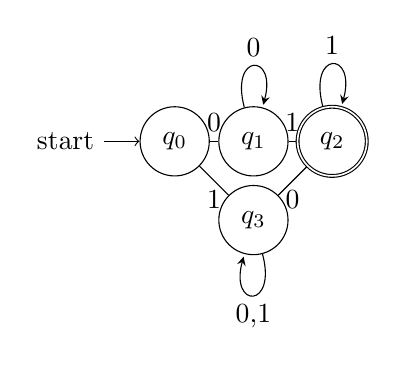
\begin{tikzpicture}
    \node[state, initial] (q0) {$q_0$};
    \node[state, right of=q0] (q1) {$q_1$};
    \node[state, accepting, right of=q1] (q2) {$q_2$};
    \node[state, below of=q1] (q3) {$q_3$};
    
    \draw [>=stealth] (q0) edge[above] node{0} (q1)
          (q0) edge[below] node{1} (q3)
          (q1) edge[loop above] node{0} (q1)
          (q1) edge[above] node{1} (q2)
          (q2) edge[below] node{0} (q3)
          (q2) edge[loop above] node{1} (q2)
          (q3) edge[loop below] node{0,1} (q3);
    \end{tikzpicture} 
    \end{center}

    The initial state of the machine is $q_0$. To check whether a word is ``accepted'' by a DFA, we simply need to follow the arrows from the initial state. This DFA works on strings of binary characters. For example, for ``001'', we would start in $q_0$, follow the arrow to $q_1$, then $q_1$ again, then to $q_2$. The inner circle for $q_2$ means that it is an \emph{accepting} state. If we end up in an accepting after processing all symbols in the input, the word is accepted by the DFA. In this case, ``001'' is accepted, but \emph{e.g.} ``0010'' would not be. In general, this DFA accepts all words comprised of one or more 0s followed by one or more 1s.

    \begin{subparts}
        \subpart[2] Define a type \haskellIn{State} which enumerates states of the DFA shown above and a type \haskellIn{Symbol} which enumerates symbols of the binary alphabet so that, for example, \haskellIn{Q0 :: State} and \haskellIn{ZERO :: Symbol}. \droppoints 
        
        \begin{solution}
            \emph{Application. 1 mark per definition.}
\begin{minted}{haskell}
data State = Q0 | Q1 | Q2 | Q3 
data Symbol = ZERO | ONE
\end{minted}
        \end{solution}
        
        \subpart[4] Define a closed type family whose kind signature is given by
        \vspace*{0.2cm}
\begin{minted}{haskell}
Delta :: State -> Symbol -> State
\end{minted}
\vspace*{0.2cm}
        and which implements transitions between states of the above DFA. For example, \haskellIn{Delta Q1 ONE} should reduce to \haskellIn{Q2}. \droppoints 
        
        \begin{solution}
            \emph{Application.}
\begin{minted}{haskell}
type family Delta (q :: Q) (e :: E) :: Q where 
    Delta Q0 ONE  = Q3 
    Delta Q0 ZERO = Q1 
    Delta Q1 ONE  = Q2 
    Delta Q1 ZERO = Q1
    Delta Q2 ONE  = Q2 
    Delta Q2 ZERO = Q3 
    Delta Q3 ONE  = Q3 
    Delta Q3 ZERO = Q3
\end{minted}
        \end{solution}
    
        \subpart[4] With the help of \haskellIn{Delta}, define a closed type family whose kind signature is given by
        \vspace*{0.2cm}
\begin{minted}{haskell}
DeltaHat :: State -> [Symbol] -> State
\end{minted}
\vspace*{0.2cm}
        and which performs transitions for every symbol in a list of symbols, starting from a given initial state. For example, the type \haskellIn{DeltaHat Q0 '[ZERO, ZERO, ONE]} should reduce to \haskellIn{Q2}. \droppoints 
        
        \begin{solution}
            \emph{Application.}
\begin{minted}{haskell}
type family DeltaHat 
    (q :: State) (e :: [Symbol]) :: State where 
    DeltaHat q '[] = q 
    DeltaHat q (e ': es) = DeltaHat (Delta q e) es
\end{minted}
        \end{solution}
    
        \ifprintanswers \else \pagebreak \fi
    
        \subpart[8] Define a closed type family whose kind signature is given by 
        \vspace*{0.2cm}
\begin{minted}{haskell}
Accepts :: State -> [State] -> [Symbol] -> Bool
\end{minted}
\vspace*{0.2cm}
        which determines whether a DFA accepts a given word. The first argument represents the initial state of the DFA, the second represents the list of final states, and the third argument represents the input word. For example, \haskellIn{Accepts Q0 '[Q2] '[ZERO, ZERO, ONE]} should reduce to \haskellIn{True}.
        \droppoints 
        
        \begin{solution}
            \emph{Application.}
\begin{minted}{haskell}
type family Elem (x :: k) (xs :: [k]) :: Bool where 
    Elem x '[]       = False 
    Elem x (x ': xs) = True 
    Elem x (y ': xs) = Elem x xs

type family Accepts 
    (q :: Q) (fs :: [Q]) (w :: [E]) :: Bool where 
    Accepts q fs w = Elem (DeltaHat q w) fs
\end{minted}
        \end{solution}
        
        \subpart[3] Define a proxy type for symbols and explain the need for proxy types in Haskell. \droppoints 
        
        \begin{solution}
            \emph{Application+Comprehension. 1 mark for definition, 2 marks for explanation.} Types in Haskell are erased during compilation once they have been checked and are therefore unavailable at run-time. As a result, functions only accept arguments whose types are of kind \haskellIn{*}. Proxy types are used to ``carry'' types of other kinds into the scope of a function's type.
            
\begin{minted}{haskell}
data SProxy (s :: Symbol) = SProxy
\end{minted}
        \end{solution}
        
        \subpart[4] Define a suitable type class and suitable type class instances to reify type-level symbols. \droppoints 
        
        \begin{solution}
            \emph{Application.} 
\begin{minted}{haskell}
class ReifySymbol (q :: E) where 
    reifySymbol :: SProxy q -> E

instance ReifySymbol ZERO where 
    reifySymbol _ = ZERO 

instance ReifySymbol ONE where 
    reifySymbol _ = ONE
\end{minted}
        \end{solution}
        
    \end{subparts}
\end{parts}
    \end{questions}
\end{document}
